%%%%%%%%%%%%%%%%%%%%%%%%%%%%%%%%%
%%% Laboratory report v2
%%% Universidad de Costa Rica
%%% Ricardo Román-Brenes
%%% ricardo.roman@ucr.ac.cr
%%%%%%%%%%%%%%%%%%%%%%%%%%%%%%%%%
\documentclass[11pt]{article}

% Document config
\usepackage[letterpaper, margin=1in]{geometry}
\usepackage[spanish]{babel}
\usepackage[utf8]{inputenc}
\usepackage{tikz}
\usepackage{hyperref}
\usepackage{color}
\usepackage{xcolor}
\usepackage{float}
\usepackage{tcolorbox}

% Color definitions
\definecolor{darkblue}{rgb}{0 , 0.054 , 0.196}
\definecolor{mygreen}{rgb}{0,0.6,0}
\definecolor{mygray}{rgb}{0.8,0.8,0.8}
\definecolor{codeBG}{rgb}{0.9, 0.97, 0.9}
\definecolor{mymauve}{rgb}{0.58,0,0.82}

\addto\captionsspanish{% Replace "english" with the language you use
  \renewcommand{\contentsname}%
    {Tabla de contenidos}%
}



\title{
{
    \begin{tikzpicture}[overlay, remember picture]
        \node[anchor=north west, %anchor is upper left corner of the graphic
            xshift=3cm, %shifting around
            yshift=-4cm] 
            at (current page.north west) %left upper corner of the page
        {
\includegraphics[height=1.3cm]{img/logoEIE.png}}; 
    \end{tikzpicture}
    \begin{tikzpicture}[overlay, remember picture]
        \node[anchor=north east, %anchor is upper left corner of the graphic
            xshift=-3cm, %shifting around
            yshift=-4cm] 
            at (current page.north east) %left upper corner of the page
        {
\includegraphics[height=1.3cm]{img/logoUCR.png}}; 
    \end{tikzpicture}
    \Large 
        \textbf{Universidad de Costa Rica}\\
        Facultad de Ingeniería\\
        Escuela de Ingeniería Eléctrica\\~\\
        \texttt{IE-0117} Programacion bajo plataformas abiertas
    }
    ~\\~\\
    {\LARGE Laboratorio 2: Usuarios, permisos y credenciales en GNU/Linux}
}
\author{M. Sc. Ricardo Román Brenes - \texttt{ricardo.roman@ucr.ac.cr}}
\date{I-2018}




\begin{document}
\maketitle


\hrule
\hrule
\tableofcontents
\hspace{5mm}
\hrule
\hrule


\section{Enunciado}




Entregue un archivo comprimido que incluya un directorio llamado informe con los archivos necesarios para generar el PDF del informe. El informe debe contener la documentacion necesaria que demuestre que se llego a una solucion satisfactorio de los problemas resueltos


\subsection{Usuarios, grupos y permisos}

\begin{enumerate}
    \item Cambie de usuario a root. sudo -s
    \item Cree un usuario nuevo llamado labo2, con la contraseña labo2.
    \item Cambie de usuario a labo2. Cree un directorio llamado PruebasPermisos en el \$HOME de este usuario.
    \item Dentro de este directorio nuevo, cree un archivo llamado README, que su contenido sea una única linea que diga: Realizando pruebas de permisos.
    \item Con un solo comando, cambie los permisos del directorio PruebasPermisos y todos los archivos que contiene, de manera tal que solamente el usuario dueno del directorio, asi como el grupo al que pertenece, tengan permisos de lectura, escritura y ejecucion. Los demas no tendran permisos de nada.
    \item Cambie a su usuario original. Trate de escribir al directorio PruebasPermisos y al archivo README contenido. Documente el resultado.
    \item Cambie de usuario a root nuevamente.
    \item Cree un grupo nuevo llamado grupolabo2, agregue el usuario labo2 y su propio usuario a este grupo.
    \item Cierre la sesion grafica de Linux y vuelva a iniciarla.
    \item Vuelva a iniciar sesion como su usuario, y cambie en terminal el usuario a labo2.
    \item Cambie recursivamente el grupo de pertenencia del directorio PruebasPermisos al grupo grupolabo2.
    \item Cierre la sesion del usuario labo2 y vuelva a su propio usuario. Trate de escribir al directorio PruebasPermisos y al archivo README. Documente el resultado.
    \item Explique con sus propias palabras el procedimiento que se realizo anteriormente. ¿Por que antes su usuario no podia escribir en el archivo? ¿Por que ahora si puede? En principio no era posible modificar con mi usuario el archivo README ni el directorio PruebasPermisos ya que solo el usuario labo2 tenia los permisos para hacerlo. Luego al crear un grupo grupolabo2 e incluir mi usuario y el usuario labo2 en este grupo, y modificar los permisos para que quienes pertenezcan al grupo puedan modificarlo, fue posibe hacer modificaciones desde mi usuario

\end{enumerate}

\subsection{Instalacion de paquetes y programas desde otros repositorios}
\begin{enumerate}
\item Siga el tutorial de instalación de Spotify en Linux que se encuentra en el siguiente enlace:
https://www.spotify.com/cr/download/linux/. Documente en su informe el porqué se
realizó cada uno de los pasos.

\end{enumerate}

\subsection{Cron, crontab, rsync, ssh}
\begin{enumerate}
\item Realice revision bibliografica de que es cron. Cron es un daemon que se ejectura desde el mismo instante en el que arranca el sistema. Comprueba si existe alguna tarea para ser ejecturada de acuerdo a la hora configurada en el sistema. En funcion de la distribucion, se inicia utilizando las carpetas /etc/rc.d/ o /etc/init.d y a cada minuto comprueba los ficheros /etc/crontab en busca de posibles ejecuciones \cite{Fulanito1999}
\item Escriba un breve resumen de cual es el formato del archivo crontab y como se utiliza. Crontab es un archivo de texto que posee una lista con todos los scripts a ejecutar. Es posible modificarlo con el comando crontab -e. \\
La estructura del comando es la siguiente: \\
min(0-59) hr(0-23) dia(0-31) mes(1-12) dia de la semana(0-6) comando a ejecutar
\item Investigue sobre el uso del comando rsync, y su uso a traves de ssh. Puede utilizar este enlace como guia https://www.digitalocean.com/community/tutorials/how-to-copy-files-with-rsync-over-ssh
\item Cree llaves ssh para su usuario de manera que no le pida contrasena a la hora de conectarse la computadora de su companero.
\item Ejecute un comando de rsync sobre ssh que permita respaldar su \$HOME en algún directorio del \$HOME del usuario de su companero.
\item Programe su computadora para realizar el ejercicio el punto anterior todos los miercoles a las 3:00am.
 
\end{enumerate}

\subsection{Instalacion de programas desde codigo fuente}
\begin{enumerate}
\item Visite el siguiente enlace: https://ffmpeg.org/download.html.
\item Descargue el fichero comprimido ffmpeg-3.4.2.tar.bz2.
\item Proceda a instalar el programa a traves del codigo fuente descargado.
Nota: recuerde revisar el README o el INSTALL para conocer las dependencias e instalarlas antes de iniciar la configuracion del paquete y la compilacion. Si no lo hace el script de configure o la compilacion podrian fallar.
\end{enumerate}






\subsection{Capturas de pantalla}


\begin{figure}[H]
\centering
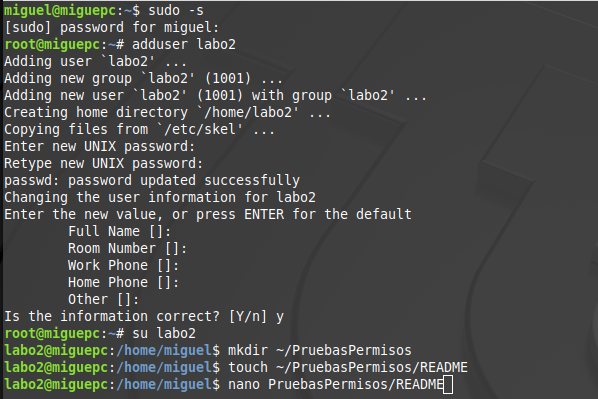
\includegraphics[width=0.5\textwidth]{img/1.png}
\caption{comandos de enunciado del 1 al 4}
\end{figure}

\begin{figure}[H]
\centering
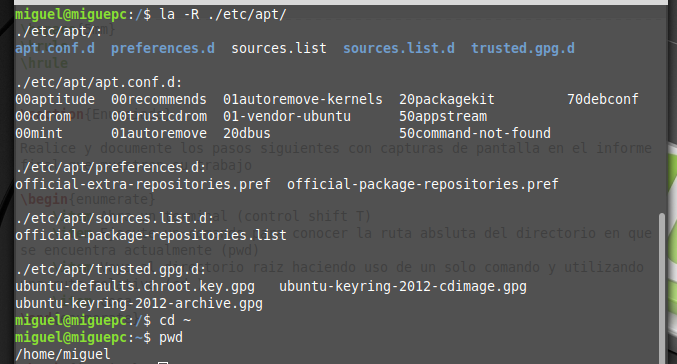
\includegraphics[width=0.5\textwidth]{img/2.png}
\caption{comandos de enunciado del 5 al 9}
\end{figure}

\begin{figure}[H]
\centering
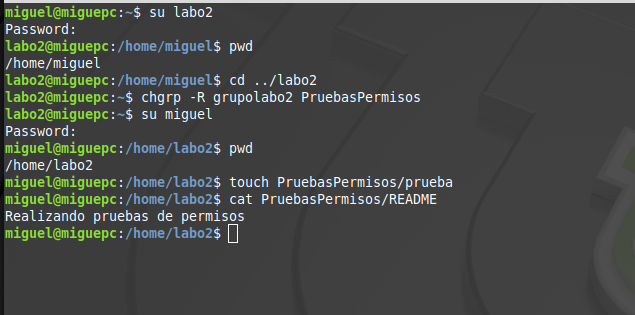
\includegraphics[width=0.5\textwidth]{img/3.png}
\caption{comandos de enunciado del 10 al 12}
\end{figure}

\begin{figure}[H]
\centering
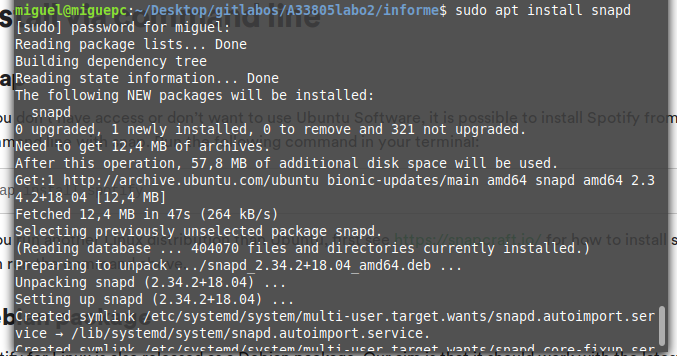
\includegraphics[width=0.5\textwidth]{img/16.png}
\caption{Instalando snapd}
\end{figure}

\begin{figure}[H]
\centering
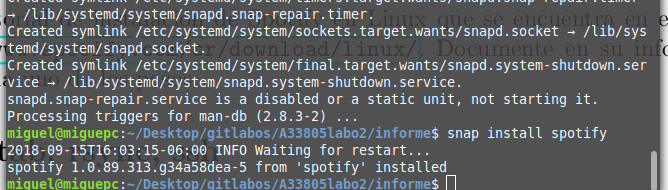
\includegraphics[width=0.5\textwidth]{img/17.png}
\caption{Instalando spotify}
\end{figure}

\begin{figure}[H]
\centering
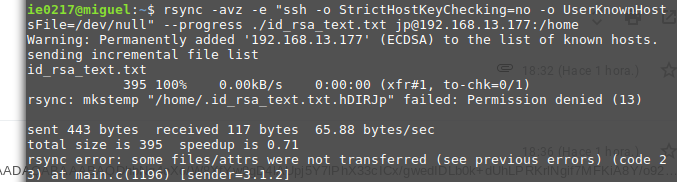
\includegraphics[width=0.5\textwidth]{img/18.png}
\caption{Uso de ssh para transferir un fichero a otra conputadora}
\end{figure}

\begin{figure}[H]
\centering
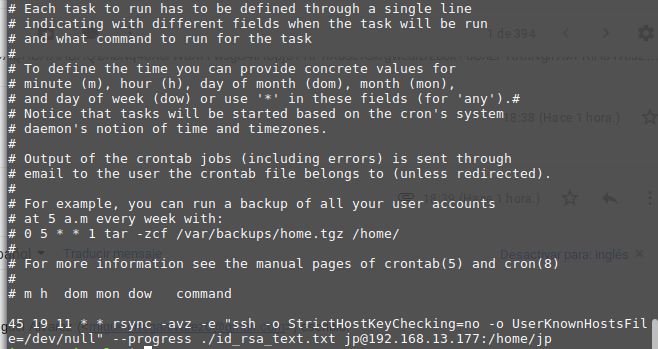
\includegraphics[width=0.5\textwidth]{img/19.png}
\caption{Uso de crontab y ssh para respaldar periodicamente un fichero a otra computadora}
\end{figure}

\begin{figure}[H]
\centering
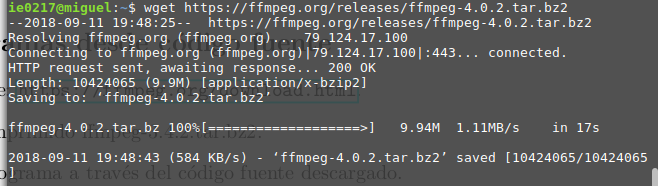
\includegraphics[width=0.5\textwidth]{img/20.png}
\caption{Instalacion de programas desde codigo fuente}
\end{figure}


\newpage
\bibliographystyle{plain}
\bibliography{2.bibliography}


\end{document}
